%!TEX root = ../thesis.tex
\chapter{Background}\label{ch:background}

This chapter will introduce core concepts from the three main fields on which this thesis draws: information theory, graph theory, and natural language processing. Throughout this thesis these three areas will be interwoven to produce new methods and results. When more specific tools from these fields are used in later chapters, they will be introduced during their discussion and this chapter referenced accordingly.

\section{Information theory}
Information theory concerns the quantitative analysis of storage and transmission of information. This field underpins much of modern information and communication technology, with applications in signal processing, data compression~\cite{schurmann1996entropy, bell1989modeling}, statistical inference~\cite{burnham_model_2002}, linguistic analysis~\cite{collobert2011natural,greenbergUniversalsLanguage1963}, cryptography~\cite{menezes2018handbook} and even human perception~\cite{delgado-bonal_human_2016}. An import concept at the heart of information theory and these applications is \emph{entropy}.

\subsection{Entropy}
Entropy is a measure of the uncertainty of a random variable. This version of entropy, commonly defined by \autoref{eq:shannon}, is referred to as Shannon entropy, named after Claude Shannon for his work in 1948 studying the quantities of information in transmitted messages~\cite{shannon_mathematical_1948}. The definitions hereafter are sourced from ``The Elements of Information Theory'' by Thomas and Cover~\cite{cover_elements_2012}.

\begin{definition}[Shannon Entropy]
	Let $X$ be a discrete random variable with alphabet $\mathcal{X}$ and probability mass function $p(x) = P(X = x), x \in \mathcal{X}$.
	The entropy $H(X)$ of $X$, is 
	\begin{equation}\label{eq:shannon}
	H(X)=-\sum_{x \in \mathcal{X}} p(x) \log_2 p(x).
	\end{equation}
\end{definition} 

The entropy of the random variable is measured in bits. A bit can have two states, 0 or 1. The entropy of a random variable is the number of bits on average that are required to describe the random variable in question. To measure the entropy in bits, we use a logarithm of base 2, and all logarithms throughout this work are assumed to be in based 2, unless otherwise specified.

To give a typical example of entropy, when an unbiased coin is tossed there are two equally probable outcomes, giving an entropy of 1 bit. 

\begin{remark}
We use the convention of $0\log 0 = 0$, which sensibly means that adding a state with 0 probably to the random variable does not change its entropy. This adds several useful properties including that the entropy is always non-negative.
\end{remark}

\begin{lemma}
	The entropy of a random variable is strictly non-negative, $H(X) \geq 0$.
\end{lemma}

\begin{proof}
	$0 \leq p(x) \leq 1$ which implies that $\log \frac{1}{p(x)} \geq 0$,
	hence the sum of products of strictly non-negative terms will always be non-negative. 
\end{proof}

\begin{remark}
	The entropy of the random variable X can also be described in terms of the \emph{expected surprise}, where the surprise of a state is $\log \frac{1}{p(x)}$.
	\begin{equation}
		H(X) = \mathbb{E} \left[ \log  \frac{1}{p(x)} \right].
	\end{equation}
\end{remark}	

An important concept we draw on throughout this work is the broader notion of \emph{complexity}. When the entropy of a system is higher, it is often said to be \emph{more complex}. While complexity itself has many varied definitions in science, we map our quantitative calculation of entropy onto this complexity, helping us discuss the impact of entropy on real systems. In essence, a more complex system is one in which one expects to be surprised more often.

\subsection{Conditional entropy and cross entropy}

The definition above for a single random variable is extended by introducing a second discrete random variable $Y$. This opens us to a variety of information theoretic quantities, only a few of which we will examine here.

We first introduce the concept of joint entropy. Joint entropy, although not directly used in the rest of this work, is a core concept when extending from a single random variable to two random variables. In essence, this joint entropy is measuring the complexity of a two dimensional probability space.

\begin{definition}[Joint Entropy]
	The joint entropy $H(X,Y)$ of a pair of discrete random variables $(X,Y)$ with a joint distribution $p(x,y)$ and state spaces $(\mathcal{X}, \mathcal{Y})$ is
	\begin{equation}\label{eq:jointentropy}
	H(X, Y)=-\sum_{x \in \mathcal{X}} \sum_{y \in \mathcal{Y}} p(x, y) \log p(x, y).
	\end{equation}
\end{definition}

This definition of joint entropy is then useful in describing conditional entropy.

\begin{definition}[Conditional Entropy]
	The conditional entropy $H(X|Y)$ of random variable $X$ given random variable $Y$ is defined as, 
		\begin{align}
		H(X | Y)&=\sum_{y \in \mathcal{Y}} p(y) H(X |Y=y) \\
		&=-\sum_{y \in \mathcal{Y}} p(y) \sum_{x \in \mathcal{X}} p(x | y) \log p(x | y) \nonumber \\ 
		&=-\sum_{y \in \mathcal{Y}} \sum_{x \in \mathcal{X}} p(x, y) \log p(x | y) \nonumber \\ 
		&=-E \log p(X | Y).
		\end{align}
\end{definition}

The conditional entropy can also be defined using the joint entropy by
\begin{equation}
H(X|Y) = H(X,Y) - H(Y).
\end{equation}
Indeed, this hints at an interpretation of conditional entropy. If the complexity of $X$ can be mostly explained by conditioning on $Y$, then the conditional entropy is very low. In a sense, this conditional entropy is hinting at a directed information relationship between the variables $X$ and $Y.$ 

Subtly different from the \emph{conditional entropy} is the \emph{cross entropy}. Whereas the \emph{conditional entropy} is the amount of information needed to describe $X$ given knowledge of $Y$, the \emph{cross entropy} is the amount of information needed to describe $X$ given a optimal coding scheme built from $Y.$ An additional subtle complication of language here is that in conditional entropy we normally refer to $X$ and $Y$ as random variables whereas cross entropy usually is directly describing relationships between \emph{distributions}. As such, we shift our notation to the distribution of $X \sim q(x)$ and $Y \sim p(y)$.

\begin{definition}[Cross Entropy]\label{def:crossentropy}
	The cross entropy $H(p||q)$ between two probability distributions, $p$ and $q$, defined over the same state space, is defined as, 
	\begin{equation}
	H (p||q)= - \sum_{x} p(x) \log {q(x)}.
	\end{equation}
\end{definition}

\begin{remark}
	Importantly, note that $H(X|Y) \neq  H(Y|X)$ and $H(p||q) \neq H (q||p)$, properties we will exploit later.
\end{remark}

The conditional entropy is a useful information-theoretic measure, but can often be difficult to compute without knowledge of the conditional probability distribution. As such, the cross entropy provides a more practical tool for us to use in our analysis.

Although cross entropy has the common notation $H(p, q)$ elsewhere in the literature, in this thesis we will use an alternative $H(p||q)$, reminiscent if the Kullback–Leibler divergence, so as to not confuse the cross entropy with the joint entropy and to provide an important notion of the direction of information flow from $q$ to $p$.

Throughout this work, entropy will be referred to in two ways. If the entropy measure in question is theoretical in nature we will use the symbols $H$, $H(X)$, or $H(X||Y)$. Where the entropy measures are estimates derived from data, we will prefer the notation $\hat{h}$, $\hat{h}(X)$, and $\hat{h}(X||Y)$. 
% The variables $X$ and $Y$ here are kept capitalised as through this work they commonly refer to a process .


So far, these entropy measures have looked at discrete random variables. There are several ways this can be extended, but as we work with sequences of random variables later, we look towards random \emph{processes} and their analysis using entropy rates.

% \subsection{Distances}
% We can extend these ideas to explore a notion of distance between probability distributions. Kullback–Leibler divergence is a measure of the inefficiency if one were to assume that a distribution is $p$ when the true distribution is $q$.

% \begin{definition}[Kullback–Leibler divergence]
% 	The Kullback–Leibler divergence (also called relative entropy), $D(p \|q)$,  between two probability distributions $p(x)$ and $q(x)$ is,
% 	\begin{align} \label{eq:kldivergence}
% 		D(p \| q) &=\sum_{x \in \mathcal{X}} p(x) \log \frac{p(x)}{q(x)} \\ 
% 					 &=E_{p} \log \frac{p(X)}{q(X)} 
% 	\end{align}
% \end{definition}

% Again, we use the convention that  $0 \log \frac{0}{0} = 0 $ and $p \log \frac{p}{0} = \infty $. 


% Conveniently, we can also express the Kullback–Leibler divergence in terms of the cross entropy.
% \begin{lemma}
% 		\begin{equation}
% 		D(p \| q) = H_p(q) - H(p) 
% 		\end{equation}
% \end{lemma}
% \begin{proof}
% 	\begin{align}
% 		D(p \| q) &=\sum_{x \in \mathcal{X}} p(x) \log \frac{p(x)}{q(x)} \\
% 		 &= \sum_{x \in \mathcal{X}} p(x) \log p(x)    -     \sum_{x \in \mathcal{X}} p(x) \log q(x)\\
% 		 &= -H(p)   +    H(q||p)\\
% 	\end{align}
% \end{proof}

% The Kullback–Leibler divergence has two difficulties; It's not symmetrical and it can return infinite values. Jensen–Shannon divergence builds from the Kullback–Leibler divergence to solve these problems to a symmetric, finite comparison between probability distributions. 

% \begin{definition}[Jensen–Shannon divergence]
%  The Jensen–Shannon divergence between two probability distributions $p(x)$ and $q(x)$ is,
% 	\begin{equation}
% 	\operatorname{JSD}(p \| q)=\frac{1}{2} D(p \| m)+\frac{1}{2} D(q \| m)
% 	\end{equation}
% 	using a mixture of the distributions, 	$m=\frac{1}{2}(p+q)$.
% \end{definition}


% \begin{remark}
% 	The square root of the Jensen–Shannon divergence provides a metric, often referred to as Jensen–Shannon distance.
% \end{remark}


\subsection{Entropy rates}\label{sec:entropyrate}

Rather than examining the entropy of a single random variable, we can turn our inquiry toward a \emph{sequence} of random variables. These random variables can be generated by some \emph{stochastic process}, which at each point in the sequence draws a realisation from a probability distribution than can depend on the previous realisations of the sequence. Consider a simple random walk where the probability distribution of the next location is centred tightly around the previous location. The future of this sequence can be said to be dependent on its past, in this case by only one time step.

In such a self-dependent stochastic process, tools such as Shannon entropy can be ineffective at fully describing the complexity. Consider two stochastic processes drawing from the set ${0,1}$: $A$ which always alternates, and $B$ which selects values randomly.

\begin{center}
\begin{tabular}{cc}
0101010101010101...  &  0001011011011100... \\ 
Sequence A & Sequence B \\
\end{tabular}
\end{center}

With knowledge of the process, we can predict perfectly that the next element of sequence $A$ is 0; whereas sequence $B$ cannot be predicted better than a coin toss. However, describing both sequences using Shannon entropy would result the same 1 bit per symbol.

The \emph{entropy rate} provides a slightly different lens for processes. The entropy rate of a stochastic process describes the amount of information required to describe the future state of a process, conditioned on the information in the history of the process.

\begin{definition}[Entropy Rate]\label{def:entropyrate}
	Let  $\mathcal{X}= \{ X_i \}$ be a ergodic stochastic process with a finite alphabet. 
	% where $X_i^j$ denotes a subsequence of the process $(X_{i}, X_{i+1}, \ldots, X_{j})$.
	The entropy rate can be defined as,
	\begin{equation}\label{eq:entropyrate}
	H(\mathcal{X})=\lim _{n \rightarrow \infty} H\left(X_{n} | X_{n-1}, X_{n-2}, \ldots, X_{1}\right).
	\end{equation}
	Given the assumption of stationarity, this can be expressed as,
	\begin{equation}
	H(\mathcal{X})=\lim _{n \rightarrow \infty} \frac{1}{n} H\left(X_{1}, X_{2}, \ldots, X_{n}\right).
	\end{equation}
\end{definition}


This entropy rate is closely connected with the ideas of compression. As noted by Kontoyiannis \emph{et al.}~\cite{kontoyiannis_nonparametric_1998}, `the entropy rate is almost surely an asymptotic lower bound on the per-symbol description length when the process is losslessly encoded'. Algorithms such as Lempel-Ziv~\cite{ziv_compression_1978} exploit these lessons to efficiently compress sequences as close to their size lower bound as practical. However, these algorithms are not a robust method of measuring the entropy rate of a sequence because implementations can differ across systems. Indeed, while this entropy is a useful theoretical tool, calculating it for real examples can prove difficult. We discuss methods of estimating entropy rates on large quantities of data in \autoref{ch:crossentropy}.

In order to assist in these later efforts, we will occasionally exploit a useful simplification of the entropy rate. If the sequence generated by a stochastic process is made from independent and identically distributed  (i.i.d.) random variables then the entropy rate of the process is simply the Shannon entropy of the random variables. 

\begin{lemma}
	The entropy rate of an i.i.d. stochastic process, $\mathcal{X}= \{ X_i \}$, is the Shannon entropy of each individual member of the process, $H(X_i)$.
\end{lemma}

\begin{proof}\label{proof:iidentroptrate}
\begin{align}
H(\mathcal{X})&=\lim _{n \rightarrow \infty} H\left(X_{n} | X_{n-1}, X_{n-2}, \ldots, X_{1}\right), \\
\intertext{and by conditional independence,}
H(\mathcal{X}) &=\lim _{n \rightarrow \infty} H\left(X_{n} \right) \nonumber \\
&= H(X_0).
\end{align}
\end{proof}

\subsection{Predictability}

Using these entropic measures we can create other quantities as well. One such useful quantity is the maximal predictability.

Predictability is the probability $\pi$ that an ideal theoretical predictive algorithm could correctly predict the next state of a process. For a process with $\pi = 0.3$, we could expect to predict this process correctly 30\% of the time. 

This $\pi$ is often difficult to obtain, however an upper bound, $\pi \leq \pi^{max}$, is possible through the use of Fano's inequality~\cite{fano_transmission_1961}.  For a process with $\pi^{max} = 0.3$, we could expect to predict this process correctly \emph{no more than} 30\% of the time, no matter how good our predictive algorithm~\cite{song_limits_2010}.


\begin{definition}[Maximal Predictability]\label{def:maximialpredictability}
For a process $X = \{ X_i \}$ with entropy $H(X)$ and state space $\mathcal{X}$, Fano's inequality in the context of our maximal predictability gives,
\begin{equation}
H(X) = H(\pi^{max}) + (1 - \pi^{max}) \log (|\mathcal{X}| - 1).
\end{equation}
\end{definition}

The entropy of the maximal predictability $H(\pi^{max})$ is substituted with the binary entropy function~\cite{song_limits_2010},   
\begin{equation}
H(\pi^{max}) = -\pi^{max} \log(\pi^{max}) - (1 -  \pi^{max}) \log(1 - \pi^{max}).
\end{equation}

Which finally gives us a form that can be solved numerically for the fundamental limit of the process predictability, $\pi^{max}$,
\begin{equation}\label{eq:predict}
-H(X)  = \pi^{max} \log(\pi^{max}) + (1 -  \pi^{max}) \log(1 - \pi^{max}) - (1 - \pi^{max}) \log (|\mathcal{X}| - 1).
\end{equation}


Throughout this thesis, maximal predictabilities will found by solving \autoref{eq:predict} using the Powell's conjugate direction method, implemented in Python using SciPy~\cite{virtanen_scipy_2019}, with a starting estimate for the root at $\pi^{max}=0.5$.

These maximal predictabilities will be used throughout this work and will be extended to a notion of maximal cross predictability in \autoref{ch:crossentropy}.


\section{Networks}

The second major area of mathematics used in this work is the theory of networks. Networks are powerful tools for encapsulating the relationships between a collection of objects~\cite{newman_networks_2018}. These objects of interest are referred as \emph{nodes}, where each node represents a distinct object. The relationships between these nodes are called \emph{edges}.

Both nodes and edges can have properties.  We differentiate here between a \emph{graph}, which is exclusively a collection of nodes and edges without extra properties, and a \emph{network}, which is a graph where nodes and edges can have properties assigned to them such that they can represent real objects. For example, a node could be a stand-in for a random variable, bundle of data or a news-media organisation. This node could have a variety of properties such as a name or Shannon entropy.

Similarly the edges can take several forms. Two nodes can have a symmetrical relationship in which they have an \emph{undirected} edge or the relationship could be \emph{directed} from one node to the other. Another important property of an edge that we use here is a \emph{weight} which can describe the magnitude of the relations between the nodes, such as the amount of flow from one node to the other.

\begin{definition}
	A network is a collection of nodes that are connected by edges. Nodes can contain meta-information and properties such as a name. Edges can have an optional direction and weight.
\end{definition}

Networks throughout this work will either be generated by using the relationships extracted from data, or relationships will be generated through a random graph model for experimentation. A random graph model is a procedure for creating a graph by following a specific algorithm, sometimes using a set of chosen parameters.  Here we outline three random graph models that will be useful in this work.

\begin{itemize}
	\item Although not random in its simplest form, we start with a clique graph~\cite{newman_networks_2018}. A clique graph is a graph where every pair of nodes has a single edge between them. When these edges are undirected, there is no randomness in this graph. However, throughout this work we will modify this clique graph such that each edge has a random direction and weight assigned to it. 
	\item One of the simplest and most widely used random network models is the Erdős–Rényi (ER) random graph model~\cite{erdos_evolution_1960,gilbert_random_1959}. This ER($n,p$) model creates a graph with $n$ nodes and links each pair of nodes with probability $p$. These graphs have an expected $n(n-1)p/2$ number of edges. Again these can take both directed and undirected forms, of which we mainly use the latter by randomly choosing a direction for each edge at its creation.
	\item Finally we introduce the more complicated Watts-Strogatz `small world' model~\cite{watts_collective_1998}. The version of the model we use imagines a set of $n$ nodes in a ring. In this ring each node has an edge connecting it to the nearest $k$ neighbours. Each of these edges is then rewired with probability $\beta$, meaning that one end of the edge is relocated to connect to a different node at random. At $\beta=0$ there is no rewiring and at $\beta=1$ the graph is approximately an ER($n,p$) graph where $p=k/(n-1)$. This $\beta$ parameter has several interesting properties; as $\beta$ increases, the average path length (the average number of hops required to get from one node to any another) decreases rapidly, the clustering coefficient decreases slowly, and the degree distribution becomes more skewed~\cite{watts_collective_1998}. As such we can change the structure of the network, without altering the total number of nodes or edges, a property we will exploit for our analysis in \autoref{ch:quotermodel}.
\end{itemize}

\begin{figure*}[!hbt]
	\centering
	\begin{subfigure}[t]{0.3\textwidth}
		\centering
		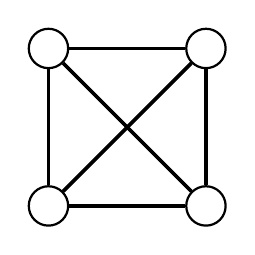
\begin{tikzpicture}[ inner sep=0mm,
		nodestyle/.style={draw, circle, fill = white, thick, minimum size=5mm},
   		edgestyle/.style={very thick}]
		\node [nodestyle] (a) at (0,0) {};
		\node [nodestyle] (b) at (2,0) {};
		\node [nodestyle] (c) at (0,2) {};
		\node [nodestyle] (d) at (2,2) {};

		\foreach \i in {a, b, c, d} 
			\foreach \j in {a, b, c, d} 
				\draw [edgestyle] (\i) -- (\j);
		\end{tikzpicture}
		\caption{}
	\end{subfigure}
	~
	\begin{subfigure}[t]{0.3\textwidth}
		\centering
		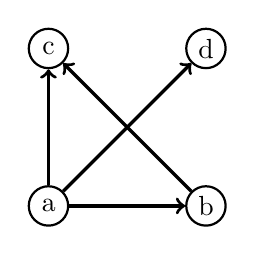
\begin{tikzpicture}[inner sep=0mm,
		nodestyle/.style={draw, circle, thick, minimum size=5mm},
   		edgestyle/.style={very thick, ->}]

		\node [nodestyle] (a) at (0,0) {a};
		\node [nodestyle] (b) at (2,0) {b};
		\node [nodestyle] (c) at (0,2) {c};
		\node [nodestyle] (d) at (2,2) {d};

 		\draw [edgestyle] (a) -- (b);
		\draw [edgestyle] (a) -- (c);
		\draw [edgestyle] (a) -- (d);
		\draw [edgestyle] (b) -- (c);
		\end{tikzpicture}
		\caption{}
	\end{subfigure}
	~
	\begin{subfigure}[t]{0.3\textwidth}
		\centering
		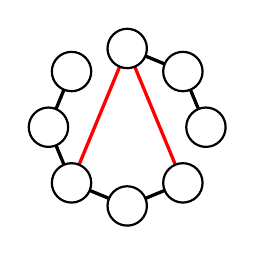
\begin{tikzpicture}[inner sep=0mm,
		nodestyle/.style={draw, circle, fill = white, thick, minimum size=5mm},
   		edgestyle/.style={very thick}]

		\foreach \angle in {0, 45,    135, 180, 225, 270   }
		{
			\draw[edgestyle] (\angle:1cm) -- ({\angle+45}:1cm);
		}

		\draw[edgestyle, red] (90:1cm) -- (225:1cm);
		\draw[edgestyle, red] (315:1cm) -- (90:1cm);

		\foreach \angle in {0, 45, ..., 315}
		{
			\node [nodestyle] (a\angle) at (\angle:1cm) {};
		}

		\end{tikzpicture}
		\caption{}
	\end{subfigure}
	\caption{Three examples of graphs and networks. (a) is an undirected clique graph with four nodes. (b) is a directed Erdős–Rényi network with four labelled nodes and $p = 2/3$. (c) is a undirected Watts-Strogatz graph with $n=8, k=2$ and $\beta=0.25$, where rewired edges are coloured red.}
	\label{fig:background_graphtypes}
\end{figure*}


While the literature is full of many diverse and useful random graph models, we choose these three models for their simplicity and ability to control specific factors. In particular, the three graphs allow us to individually control the network size, edge probability and rewiring complexity independently, while holding other parameters constant. This allows us to examine the relationship between graph properties in several settings and their flow dynamics, which we study in \autoref{ch:quotermodel}.

Some example graphs and networks are shown in \autoref{fig:background_graphtypes}. By combining these tools with information theory, we can construct networks from data and simulate information flows through networks, but a final tool-kit is needed to process the raw data we are interested in.


\section{Natural language processing}

While information theory and networks will form a backbone of our analysis, the data we are interested in comes in a difficult form. Natural language is the non-rigid, semi-unstructured style of language used in everyday conversation and writing. This natural language is the type of text that makes up the social media news of interest to us. In order to study this and convert it to useful forms for quantitative analysis we need an additional tool-kit.

Natural language processing (NLP) is the area of study in which unstructured human language is examined via machine. Formally, natural language refers to either spoken or written language, designed to be understandable to a human listener or reader. This language is not explicitly designed to be machine understandable, and machine comprehension of this language is a challenging problem~\cite{baeza-yates_challenges_2004}.

NLP is a broad term covering many models and techniques for computationally processing meaningful information from text, ranging from the simple identification of individual words, to the extraction of deeper semantic meaning. 

Early work in NLP focused around simple grammatical rules and small vocabularies, such as the work of Georgetown-IBM~\cite{hutchins_first_1997} to translate 60 sentences from Russian to English in 1954. With the rapid increase in computational power and the size of digital text corpora, modern NLP has focused on deeper challenges of extracting meaning from text with tools such as Word2Vec~\cite{mikolov_distributed_2013, mikolov_efficient_2013} or deep learning methods such as Google's BERT~\cite{devlin_bert_2019}.

These methods face a daunting challenge: language is not only complex and often duplicitous, but contextual and ever-changing. In this work, we present a new comparative method of natural language processing, which attempts to implicitly build this context into the network it creates.

\subsection{Tokenization}\label{sec:tokenization}
The first step of any natural language processing is tokenization. Tokenization is the fundamental building block of NLP and can often prove deceptively hard. In simple terms, tokenizing a piece of text is the process of breaking a long sequence of characters into smaller chucks of characters called tokens. This often means breaking a sentence into words, \emph{e.g.} \texttt{`This thesis is great' } becomes \texttt{[`This', `thesis', `is',  `great']}.

The task becomes more complex when we introduce contractions. In the case of the word, \texttt{``that's''}, should we introduce a new token to represent the compound, or break it into two new tokens, \texttt{[`that', `is']}? There are many such choices that can be made during tokenization and several will be discussed when they are applied in \autoref{ch:data}.

While each choice may seem trivial, a process of matching segments of text is highly dependent on tokenization choices such as these, which will have carry on effects to the rest of this work. While there are many aspects of tokenisation that could be elaborated upon here, we focus on one very simple and important concept, the vocabulary size, as it will be critically important throughout this thesis. 

% \ts{There is much more I could add here (\emph{e.g.} compound words, dealing with unknown characters, the comparison of character level vs word level tokens, unsupervised learning of tokenization (very cool)) but I feel that these are not relevant and worth leaving out.}

\subsubsection{Vocabulary size}\label{sec:background_vocab_sizes}

% One such impact of tokenization choices is the vocabulary size of a text corpus. 

The vocabulary size is simply the number of unique tokens in any corpus. In general, the vocabulary size of a corpus grows sub-linearly with the total number of tokens~\cite{heaps1978information}. This is deeply important to our work as an increased vocabulary size can often result in a larger complexity. Given the differences in data collection and content production, we sometime have need to observe the complexity of the language independent of the vocabulary size or token count. As such, vocabulary is a fundamental properly which we referenced throughout this work.

\subsection{Text generation}\label{sec:textgeneration}

Text generation, sometimes referred to as natural-language generation, is an algorithmic process of generating natural-looking text. Text generation has many applications from chat-bots~\cite{MauldinChatterbots1994} and article writing bots to text generation for modelling and analysis purposes~\cite{Touseefsurvey2020}.

The techniques range from dictionary approaches, such as those first used by ELIZA in 1964~\cite{weizenbaum_computer_1976}, to language models which can range from simple probabilist generators~\cite{reiter2000building} to large machine learned models trained on huge quantities of text~\cite{perera2017recent}. Each generation approach has trade-offs, especially with regards to explainability. Large complex models based on deep learning can prove extremely effective and powerful, but post risks in scientific settings when models are stochastically trained ``black boxes'' with results that are not reproducible.

In scientific settings such as this work, it is often best to apply simple models, even at the expense of realism. One such model we use throughout this work is a simple independent and identically distributed (i.i.d.) generation approach. This approach repeatedly draws from a bag of tokens with replacement according to a chosen distribution. 

\subsubsection{Zipf's law}
One such example is drawing from a Zipf distribution~\cite{george1935zipf,zipf_human_1949}. This distribution is based on results from quantitative linguistics showing that in many corpora of natural language the frequency of words is inversely proportional to a power of their rank in the list of most frequent words. This is closely related with a power-law distribution, and can be stated mathematically as the probability of a word with rank $k$ occurring next being,
\begin{equation}
P(k) = \frac{1}{k^\alpha}\frac{1}{H_{V,\alpha}},
\end{equation}
where $V$ is the total vocabulary size, $\alpha$ is scaling parameter characterizing the distribution and $H_{V,s}$ is the $V$th generalised harmonic number which acts as a normalising constant. 

The choice of $\alpha$ in such a distribution is usually derived from fitted data. As various results for $\alpha$ exist between different corpses (usually ranging from between 0.5 to 2), we will fit the scaling parameter on our own data in \autoref{sec:zipf_fit}.

\subsubsection{Alternative approaches}
While many other approaches for synthetic text generation exist we restrain ourselves to these i.i.d. models listed here. 

More complex models can produce very realistic text, for instance through deep learning techniques, however it is impossible analytically compute entropy rates for these models. Conversely, simpler models such as Markov chain text generation do have analytic entropy rates, but require more assumptions to be made about the text process in creating the transition probabilities. 

We find here that the Zipf i.i.d. model sufficiently balances realism for our context while requiring only a single parameter to be fit. Indeed, when we use this text generation we will also apply the same techniques to real text data in \autoref{ch:crossentropy} and \autoref{ch:quotermodel} and find similar results. 


In this chapter, we have introduced three mathematical fields separately. However, moving forward -- and especially in \autoref{ch:quotermodel} -- we will be combining these areas to produce hybrid tools (\emph{e.g.}  natural language generation on networks to produce information flows). First, these tools require data, a topic we now turn out attention to in \autoref{ch:data}

